% !TEX root = main.tex

%%%-------------------------------------------
\section{Алгоритм обратного распространения ошибки}

\epigraph{Что происходит, когда мы суём пальцы в розетку? Нас бьёт током! Мы делаем ошибку, и она распространяется по нашему телу.}{\textit{Твоя мама}}


%%%-------------------------------------------
\begin{problem}{(граф вычислений)}
    Как найти производную $a$ по $b$ в графе вычислений? Находим не посещённый путь из $a$ в $b$, перемножаем все производные на рёбрах получившегося пути. Добавляем это произведение в сумму. Так делаем для всех путей. 
    
    Маша хочет попробовать этот алгоритм на функции
    
    $$
    f(x,y) = x^2 + xy + (x + y)^2.
    $$ 
    
    Помогите ей нарисовать граф вычислений и найти $\frac{\partial f}{\partial x}$ и $\frac{\partial f}{\partial y}.$ В каждой вершине графа записывайте результат вычисления одной элементарной операции: сложений или умножения. 
    
    граф вычислений. В вершинах графа она будет записывать результаты вычислений. Каждое ребро будет обозначать элементарную операцию: плюс или умножить\footnote{По мотивам книги Николенко "Глубокое обучение" (стр. 79)}.
\end{problem} 

\begin{sol}  Нарисуем граф вычислений. 
\begin{center}
    \begin{tikzpicture}
        \tikzstyle{place}=[draw=black,ellipse,minimum height=20pt,minimum width=50pt,inner sep=2pt]
        
        \draw node at (0, 0) [place] (x) {$x$};
        \draw node at (4, 0) [place] (y) {$y$};
        \draw node at (-2, 2) [place] (a) {$a = x^2$};
        \draw node at (1, 2) [place] (b) {$b = x \cdot y$};
        \draw node at (5, 2) [place] (c) {$c = x + y$};
        \draw node at (-1, 4) [place] (d) {$d = a + b$};
        \draw node at (3, 4) [place] (e) {$e = c^2$};
        \draw node at (1, 6) [place] (f) {$f = d + e$};
        
        \draw [->]  (x) to (a);
        \draw [->]  (x) to (b);
        \draw [->]  (x) to (c);
        \draw [->]  (y) to (b);
        \draw [->]  (y) to (c);
        \draw [->]  (a) to (d);
        \draw [->]  (b) to (d);
        \draw [->]  (c) to (e);
        \draw [->]  (e) to (f);
        \draw [->]  (d) to (f);
    \end{tikzpicture}
\end{center}

Каждому ребру припишем производную выхода по входу. Например, ребру между $x$ и $a$ будет соответствовать $\frac{\partial a}{\partial x} = 2x.$

\begin{center}
    \begin{tikzpicture}
        \tikzstyle{place}=[draw=black,ellipse,minimum height=20pt,minimum width=50pt,inner sep=2pt]
        
        \draw node at (0, 0) [place] (x) {$x$};
        \draw node at (4, 0) [place] (y) {$y$};
        \draw node at (-2, 2) [place] (a) {$a = x^2$};
        \draw node at (1, 2) [place] (b) {$b = x \cdot y$};
        \draw node at (5, 2) [place] (c) {$c = x + y$};
        \draw node at (-1, 4) [place] (d) {$d = a + b$};
        \draw node at (3, 4) [place] (e) {$e = c^2$};
        \draw node at (1, 6) [place] (f) {$f = d + e$};
        
        \draw [->, red]  (x) to (a) node[below=1.cm] {$\frac{\partial a}{\partial x} = 2x$};
        \draw [->, red, dashed]  (x) to (b) node[below=10.mm, left] {$\frac{\partial b}{\partial x} = y$};
        \draw [->, amethyst, thick]  (x) to (c) node[below=9mm, left] {$\frac{\partial c}{\partial x} = 1$};
        \draw [->]  (y) to (b) node[below=9.mm, right] {$\frac{\partial b}{\partial y} = x$};
        \draw [->]  (y) to (c) node[below=8.mm, right] {$\frac{\partial c}{\partial y} = 1$};
        \draw [->, red]  (a) to (d) node[below=10.mm, left] {$\frac{\partial d}{\partial a} = 1$};
        \draw [->, red, dashed]  (b) to (d) node[below=10.mm, right] {$\frac{\partial d}{\partial b} = 1$};
        \draw [->, amethyst, thick]  (c) to (e) node[below=10.mm, right] {$\frac{\partial e}{\partial c} = 2c$};
        \draw [->, amethyst, thick]  (e) to (f) node[below=10.mm, right] {$\frac{\partial f}{\partial e} = 1$};
        \draw [->, red]  (d) to (f) node[below=10.mm, left] {$\frac{\partial f}{\partial d} = 1$};
    \end{tikzpicture}
\end{center}

Теперь пройдём по всем траекториям из $x$ в $f$ и перемножим производные на рёбрах. После просуммируем получившиеся множители 

\begin{multline*}
\frac{\partial f}{\partial x} = \frac{\partial f}{\partial d} \cdot \frac{\partial d}{\partial a} \cdot \frac{\partial a}{\partial x} + \frac{\partial f}{\partial d} \cdot \frac{\partial d}{\partial b} \cdot \frac{\partial b}{\partial x} + \frac{\partial f}{\partial e} \cdot \frac{\partial e}{\partial c} \cdot \frac{\partial c}{\partial x} = \\ =  1 \cdot 1 \cdot 2x + 1 \cdot 1 \cdot y + 1 \cdot 2c \cdot 1 = 2x + y + 2(x + y).
\end{multline*}

По аналогии найдём производную по траекториям из $y$ в $f$:

\[
\frac{\partial f}{\partial y} =  1 \cdot 1 \cdot x +  1 \cdot 2c \cdot 1 = x + 2(x + y).
\]
\end{sol} 


%%%-------------------------------------------
\begin{problem}{(придумываем backpropagation)} 
У Маши есть нейросеть с картинки ниже, где $w_{ij}^k$ --- веса для $k$ слоя, $f(t)$ --- какая-то функция активации. Маша хочет научиться делать для такой нейронной сетки градиентный спуск.

    \begin{center}
    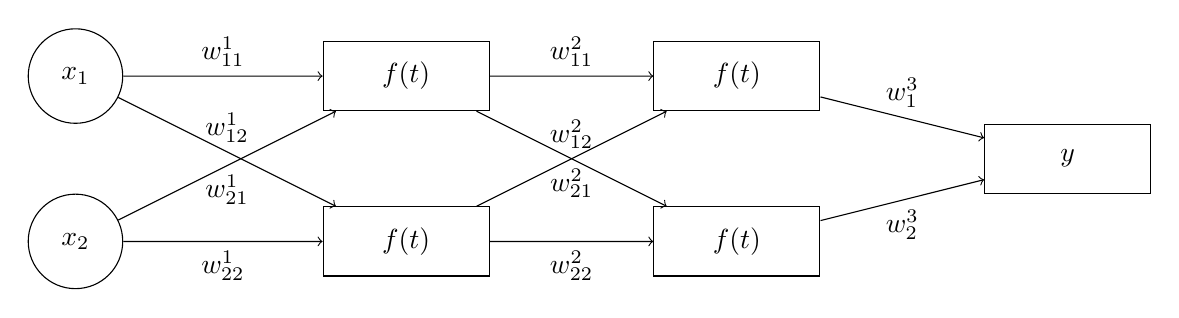
\begin{tikzpicture}[scale=1.4]
    	\tikzstyle{place}=[circle, draw=black, minimum size = 12mm]
    	\tikzstyle{placeh}=[draw=black, minimum height=25pt,minimum width=60pt,inner sep=2pt]
    	
    	% Input
    	\foreach \x in {1,...,2}
    	\draw node at (0, -\x*1.5) [place] (first_\x) {$x_\x$};
    	
    	% Hidden 1
    	\foreach \x in {1,...,2}
    	\node at (3, -\x*1.5) [placeh] (second_\x){$f(t)$};		
    	
    	% Hidden 2
    	\foreach \x in {1,...,2}
    	\node at (6, -\x*1.5) [placeh] (third_\x){$f(t)$};	
    	
    	% Output
    	\node at (9, -2.25) [placeh] (fourth){$y$};
    	
    	\draw [->]  (first_1) to node[above]{$w_{11}^1$} (second_1);
    	\draw [->]  (first_1) to node[above]{$w_{12}^1$} (second_2);
    	\draw [->]  (first_2) to node[below]{$w_{21}^1$} (second_1);
    	\draw [->]  (first_2) to node[below]{$w_{22}^1$} (second_2);
    	
    	\draw [->]  (second_1) to node[above]{$w_{11}^2$} (third_1);
    	\draw [->]  (second_1) to node[above]{$w_{12}^2$} (third_2);
    	\draw [->]  (second_2) to node[below]{$w_{21}^2$} (third_1);
    	\draw [->,]  (second_2) to node[below]{$w_{22}^2$} (third_2);
    	
    	\draw [->]  (third_1) to node[above]{$w_1^3$} (fourth);
    	\draw [->]  (third_2) to node[below]{$w_2^3$} (fourth);
    \end{tikzpicture}
    \end{center} 
    
    \begin{enumerate}
        \item  Запишите Машину нейросеть, как сложную функцию. Сначала в виде нескольких уравнений, а затем в матричном виде. 
    	
    	\item Предположим, что Маша решает задачу регрессии. Она прогоняет через нейросетку одно наблюдение. На выходе она вычисляет знчение функции потерь $L(W_1, W_2, W_3) = \frac{1}{2} \cdot (y - \hat y)^2$ --- функция потерь, где $W_k$ --- веса $k-$го слоя.  Найдите производные функции $L$ по всем весам $W_k$. 
    	
    	\item В производных постоянно повторяются одни и те же части. Постоянно искать их не очень оптимально. Выделите эти часть в прямоугольнички цветными ручками. 
    	
    	\item Выпишите все производные в том виде, в котором их было бы удобно использовать для алгоритма обратного распространения ошибки, а затем, сформулируйте сам алгоритм. Нарисуйте под него удобную схемку.
    \end{enumerate}
\end{problem}

\begin{sol} Договоримся до следующих обозначений. Буквами $h^k_{ij}$ будем обозначать выход $k-$го слоя для $j-$го нейрона для $i-$го наблюдения до применения функции активации. Буквами  $o^k_{ij}$ будем обозначать всё то же самое после применения функции активации. Например, для первого слоя:

\begin{equation*}
    \begin{aligned} 
    & h^1_{i1} = w^1_{11} \cdot x_{i1} +  w^1_{21} \cdot x_{i2} \\
    & o^1_{i1} = f(h_{i1}^1). \\
    \end{aligned} 
\end{equation*}

\indef{Делай раз.} Для начала перепишем сетку в виде нескольких уравнений. Для первого слоя мы находим
\begin{equation*}
    \begin{aligned} 
    & o^1_{i1} = f( w^1_{11} \cdot x_{i1} +  w^1_{21} \cdot x_{i2}) \\
    & o^1_{i2} = f( w^1_{12} \cdot x_{i1} +  w^1_{22} \cdot x_{i2}). \\
    \end{aligned} 
\end{equation*}

Для второго работают аналогичные уравнения, но значения $x$ заменяются на соответствующие $o$. На выходе мы предсказываем $y$, как взвешенную суммы выходов со второго слоя
\[
\hat{y}_i = w_1^3 \cdot o^2_{i1} + w_2^3 \cdot o^2_{i2}.
\]

Подставим вместо $o^2_{1i}$ и $o^2_{2i}$ результат вычисления предыдущих слоёв
\[
\hat{y}_i = w_1^3 \cdot f( w^1_{12} \cdot o^1_{i1} +  w^1_{22} \cdot o^1_{i2}) + w_2^3 \cdot f( w^1_{12} \cdot o^1_{i1} +  w^1_{22} \cdot o^1_{i2}).
\]

Подставим результат вычисления первого слоя 
\begin{multline*}
\hat{y}_i = w_1^3 \cdot f( w^1_{12} \cdot f( w^1_{11} \cdot x_{i1} +  w^1_{21} \cdot x_{i2}) +  w^1_{22} \cdot f( w^1_{12} \cdot x_{i1} +  w^1_{22} \cdot x_{i2})) + \\ + w_2^3 \cdot f( w^1_{12} \cdot f( w^1_{11} \cdot x_{i1} +  w^1_{21} \cdot x_{i2}) +  w^1_{22} \cdot f( w^1_{12} \cdot x_{i1} +  w^1_{22} \cdot x_{i2})).
\end{multline*}

Мы записали нашу нейросеть в виде сложной функции. Выглядит ужасно. 

Давайте перепишем всё то же самое более компактно, в матричном виде. Начнём с первого слоя. На самом деле, чтобы найти строчку $(h^1_{i1}, h^1_{i2})$ мы делаем матричное умножение. Строчку $(x_{i1},  x_{i2})$ мы умножаем на матрицу весов $W_1$

\begin{equation*} 
    \begin{pmatrix} h^1_{i1} & h^1_{i2} \end{pmatrix} =  \begin{pmatrix} x_{i1} &  x_{i2}\end{pmatrix} \cdot \begin{pmatrix} w^1_{11} &  w^1_{12} \\ w^1_{21} & w^1_{22}\end{pmatrix}.
\end{equation*} 

Чтобы получить $h_1$ мы умножаем строчку из переменных на первый столбец, чтобы получить $h_2$, на второй столбец. Получается, что в терминах матриц каждый нейрон нашей сети это столбец. Если мы добавим ещё один столбец из весов в матрицу, это будет эквивалентно добавлению в сетку третьего нейрона, так как на выходе мы будем получать ещё и $h_3$. Если у нас появится дополнительный вход $x_3$, в матрицу нам нужно будет добавить ещё одну строчку из весов. 

Запишем первый слой в матричном виде. На вход идёт матрица из наблюдений $X_{[n \times 2]}$, она умножается на матрицу весов $W_{[2 \times 2]}$, получается матрица $H_{[n \times 2]}$. Ко всем элементам этой матрицы мы применяем функцию активации $f$. Делаем это поэлементно

\[
O_1 = f(H_1) = f(X\cdot W_1).
\]

Остальные слои записываются по аналогии. Получается, что наша нейросеть в матричном виде выглядит как 

\[
\hat{y} = f(f(X\cdot W_1) \cdot W_2) \cdot W_3.
\]

Здесь $\hat{y}$ --- вектор столбец размера $[n \times 1]$, а матрицы весов обладают размерностями $[2 \times 2]$, $[2 \times 2]$ и $[2 \times 1]$ соответственно. 
 
\indef{Делай два,} выписываем функцию потерь и аккуратно берём все производные

\[
L(W_1, W_2, W_3) = \frac{1}{2} \cdot (y - \hat y)^2 = \frac{1}{2} \cdot (y - f(f(x \cdot W_1) \cdot W_2) \cdot W_3)^2.
\]


\todo[inline]{Бляяяя}


Здесь $y$ это скаляр, а $x$ это строчка. Всего нам надо взять три матричные производные. Функция $h = x \cdot A$  бьёт из векторов $[1 \times 2]$ в вектора $[1 \times 2]$. Значит 


С транспонированием около матриц надо просто смириться. Мы используем правило взятия матричных производных, которое состоит в том, что для  производная $\frac{\partial f}{\partial X} = A^T$. Обычно мы работаем с векторами-столбцами и это нужно, чтобы с размерностями матриц не возникало проблем. Если хочется разобраться подробнее, прочитайте необязательную часть про матричное дифференцирование. 




Просто делаем это по правилу взятия производной сложной функции. Как в школе. 

\begin{equation*}
    \begin{aligned} 
    & \underset{[2 \times 1] }{\frac{\partial L}{\partial W_3}} =  \frac{\partial L}{\partial \hat y} \cdot \frac{\partial \hat y}{\partial W_3} =  \underset{[1 \times 1] }{(y - \hat{y})}  \cdot f(f(x\cdot W_1) \cdot W_2) \\
    & \frac{\partial L}{\partial W_2} =  \frac{\partial L}{\partial \hat y} \cdot \frac{\partial \hat y}{\partial W_2} =  (y - \hat{y}) \cdot  W_3 \cdot f'(f(x\cdot W_1) \cdot W_2) \cdot f(x\cdot W_1) \\
    & \frac{\partial L}{\partial W_1} = \frac{\partial L}{\partial \hat y} \cdot \frac{\partial \hat y}{\partial W_1} =  (y - \hat{y})  \cdot  W_3 \cdot f'(f(x\cdot W_1) \cdot W_2) \cdot W_2 \cdot  f'(x\cdot W_1) \cdot X \\
    \end{aligned} 
\end{equation*}

Проследим за размером всех производных.

Выделим в прямоугольники части, которые каждый раз считаются заново, хотя могли бы переиспользоваться. 


\begin{equation*}
    \begin{aligned} 
    & \frac{\partial L}{\partial W_3} =  \frac{\partial L}{\partial \hat y} \cdot \frac{\partial \hat y}{\partial W_3} = \boxed{ (y - \hat{y}) } \cdot f(f(x\cdot W_1) \cdot W_2) \\
    & \frac{\partial L}{\partial W_2} =  \frac{\partial L}{\partial \hat y} \cdot \frac{\partial \hat y}{\partial W_2} = \boxed{ (y - \hat{y})} \cdot \boxed{ W_3 \cdot f'(f(x\cdot W_1) \cdot W_2)} \cdot f(x\cdot W_1) \\
    & \frac{\partial L}{\partial W_1} = \frac{\partial L}{\partial \hat y} \cdot \frac{\partial \hat y}{\partial W_1} = \boxed{ (y - \hat{y}) } \cdot \boxed{ W_3 \cdot f'(f(x\cdot W_1) \cdot W_2)} \cdot W_2 \cdot  f'(x\cdot W_1) \cdot X \\
    \end{aligned} 
\end{equation*}

Если бы слоёв было бы больше, переиспользования возникали бы намного чаще. Градиентный спуск при таком подходе мы могли бы сделать точно также, как и в любых других моделях \begin{equation*}
    \begin{aligned} 
    & W_3^t = W_3^{t-1} - \eta \cdot \frac{\partial L}{\partial W_3}( W_3^{t-1}) \\
    & W_2^t = W_2^{t-1} - \eta \cdot\frac{\partial L}{\partial W_2} ( W_2^{t-1}) \\
    & W_1^t = W_1^{t-1} - \eta \cdot\frac{\partial L}{\partial W_1} ( W_1^{t-1}).
    \end{aligned} 
\end{equation*}

Проблема в том, что такой подход из-за постоянных перевычислений будет работать долго. Алгоритм обратного распространения ошибки помогает более аккуратно считать производную и ускорить обучение нейросетей. 

\indef{Делай три,} выпишем алгоритм обратного распространения ошибки в виде красивой схемки. Сначала мы делаем прямой проход по нейросети (forward pass): 

\begin{center}
	\begin{tikzpicture}
	\tikzstyle{place}=[rectangle, draw=black, minimum size = 8mm]
	\draw node at (0, 0) (input) {$\underset{[n \times 2]}{X}$};
	\draw node at (2, 0) (h1) {$\underset{[n \times 2]}{H_1}$};
	\draw node at (4, 0) (o1) {$\underset{[n \times 2]}{O_1}$};
	\draw node at (6, 0) (h2) {$\underset{[n \times 2]}{H_2}$};
	\draw node at (8, 0) (o2) {$\underset{[n \times 2]}{O_2}$};
	\draw node at (10, 0) (output) {$\underset{[n \times 1]}{\hat{y}} $};
	\draw node at (12, 0) (mse) {$L(y, \hat y)$};
	
	\draw [->]  (input) -- (h1) node[pos=.49, above] {$\underset{[2 \times 2]}{W_1}$} ;
	\draw [->]  (h1) -- (o1) node[pos=.49, above] {$f$} ;
	\draw [->]  (o1) -- (h2) node[pos=.49, above] {$\underset{[2 \times 2]}{W_2}$} ;
	\draw [->]  (h2) -- (o2) node[pos=.49, above] {$f$} ;
	\draw [->]  (o2) -- (output) node[pos=.49, above] {$\underset{[2 \times 1]}{W_3}$} ;
	\draw [->]  (output) to (mse);	
	\end{tikzpicture}
\end{center}

Под всеми матрицами подписаны размерности. Взятие функции активации --- поэлементная операция, она никак не меняет размер матрицы. Это будет важно при взятии производных. В ходе прямого прохода мы запоминаем все промежуточные результаты. Они нам пригодятся для поиска производных при обратном проходе. Например, $\frac{\partial H_2}{\partial W_2} = O_2^T.$ Получается, в какой-то момент нам надо будет переиспользовать результаты вычислений, полученных при прямом проходе.



Наша нейросеть --- граф вычислений. Давайте запишем для каждого ребра в рамках этого графа производную. Везде под производными подпишем размерности соотвествующих матриц

\begin{center}
	\begin{tikzpicture}
		\draw node at (0, 0) (input) {$X$};
		\draw node at (2, 0) (h1) {$H_1$};
		\draw node at (4, 0) (o1) {$O_1$};
		\draw node at (6, 0) (h2) {$H_2$};
		\draw node at (8, 0) (o2) {$O_2$};
		\draw node at (10, 0) (output) {$\hat{y} $};
		\draw node at (12, 0) (mse) {$MSE$};
		
		\draw [->, dashed]   (h1)  -- (input) node[pos=.49, above] {$\frac{\partial H_1}{\partial X}$} ;
		\draw [->, dashed]   (o1) -- (h1) node[pos=.49, above] {$\frac{\partial O_1}{\partial H_1}$} ;
		\draw [->, dashed]   (h2) -- (o1) node[pos=.49, above] {$\frac{\partial H_2}{\partial O_1}$} ;
		\draw [->, dashed]   (o2) -- (h2) node[pos=.49, above] {$\underset{[n \times 2]}{\frac{\partial O_2}{\partial H_2}}$} ;
		\draw [->, dashed]   (output) -- (o2)node[pos=.49, above] {$\underset{[n \times 2]}{\frac{\partial \hat{y}}{\partial O_2}}$} ;
		\draw [->, dashed]  (mse) -- (output) node[pos=.49, above] {$\underset{[1 \times n]}{ \frac{\partial L}{\partial \hat{y} } }$} ;	
		
		\draw [->, dashed]  (9, -0.05) -- (9, -1.2)  node[pos=.49, right] {$\frac{\partial \hat{y}}{\partial W_3} = \underset{[n \times 2]}{O_2}$} ;
		\draw [->, dashed]  (5, -0.05) -- (5, -1.2)  node[pos=.49, right] {$\frac{\partial H_2}{\partial W_2} = O_1$} ;
		\draw [->, dashed]  (1, -0.05) -- (1, -1.2)  node[pos=.49, right] {$\frac{\partial H_1}{\partial W_1} = X$} ;
	\end{tikzpicture}
\end{center}

Осталось только аккуратно записать обратный ход алгоритма. Заведём для накопленного значения производной переменную $d$. На первом шаге нам надо найти $\frac{\partial L}{\partial W_3}$. Сделаем это в два хода

\begin{equation*} 
	\begin{aligned}
		&  d = \frac{\partial L}{\partial \hat y} \\
		&  \frac{\partial L}{\partial W_3} = d \cdot O_2^T.
	\end{aligned}
\end{equation*}

Вектор $d$ будет размера $[n \times 1]$, матрица $O_2^T$ будет размера 



Для поиска производной $\frac{\partial L}{\partial W_2}$ переиспользуем значение, которое накопилось в $d$. Нам надо найти 

\[
\frac{\partial L}{\partial W_2} = \frac{\partial L}{\hat y} \cdot \frac{\partial \hat y}{\partial O_2} \cdot \frac{\partial O_2}{\partial H_2} \cdot \frac{\partial H_2}{\partial W_2} = d \cdot \boxed{ \frac{\partial \hat y}{\partial O_2} \cdot \frac{\partial O_2}{\partial H_2} } \cdot \frac{\partial H_2}{\partial W_2}.
\]

Часть, выделенную в прямоугольник мы будем переиспользовать для поиска $\frac{\partial L}{\partial W_1}$. Хорошо бы дописать её в $d$ для этого. Получается, вторую производную тоже надо найти в два хода

\begin{equation*} 
	\begin{aligned}
		&  d = d \cdot \frac{\partial \hat y}{\partial O_2} \cdot \frac{\partial O_2}{\partial H_2} \\
		&  \frac{\partial L}{\partial W_2} = d \cdot O_1.
	\end{aligned}
\end{equation*}

Осталась заключительная производная $\frac{\partial L}{\partial W_1}$. Нам надо найти 

\[
\frac{\partial L}{\partial W_2} = \frac{\partial L}{\hat y} \cdot \frac{\partial \hat y}{\partial O_2} \cdot \frac{\partial O_2}{\partial H_2} \cdot \frac{\partial H_2}{\partial O_1} \cdot \frac{\partial O_1}{\partial H_1}  \cdot \frac{\partial H_1}{\partial W_1}  = d \cdot \frac{\partial H_2}{\partial O_1} \cdot \frac{\partial O_1}{\partial H_1}  \cdot \frac{\partial H_1}{\partial W_1}.
\]

Снова делаем это в два шага

\begin{equation*} 
	\begin{aligned}
		&  d = d \cdot  \frac{\partial H_2}{\partial O_1} \cdot \frac{\partial O_1}{\partial H_1} \\
		&  \frac{\partial L}{\partial W_1} = d \cdot X.
	\end{aligned}
\end{equation*}

Если бы нейросетка была бы глубже, мы смогли бы переиспользовать $d$ на следующих слоях. Каждую производную благодаря такому постепенному подходу мы нашли ровно один раз. Это и есть алгоритм обратного распространения ошибки. 
\end{sol} 


%%%-------------------------------------------
\begin{problem}{(Backpropagation без константы)} 
У Маши есть нейросеть с картинки ниже. Она использует функцию потерь  $L(W_1, W_2, W_3) = \frac{1}{2} \cdot (y - \hat y)^2$. В качестве функции активации Маша выбрала сигмоиду $\sigma(t) = \frac{e^t}{1 + e^t}$.

    \begin{center}
    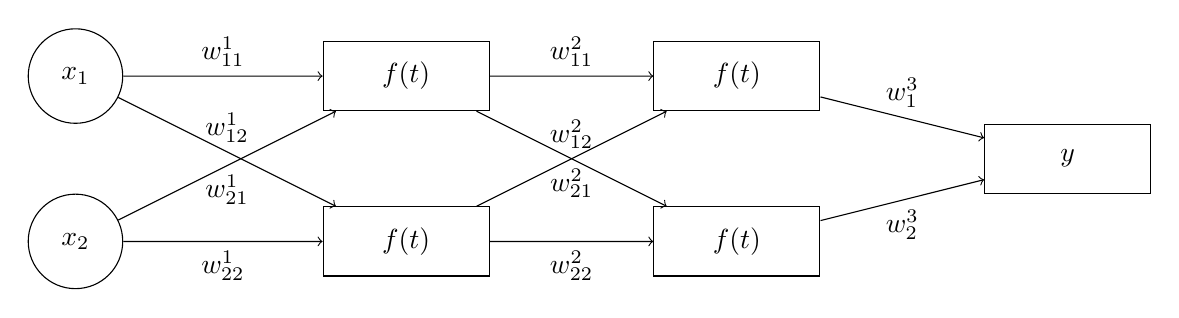
\begin{tikzpicture}[scale=1.4]
    	\tikzstyle{place}=[circle, draw=black, minimum size = 12mm]
    	\tikzstyle{placeh}=[draw=black, minimum height=25pt,minimum width=60pt,inner sep=2pt]
    	
    	% Input
    	\foreach \x in {1,...,2}
    	\draw node at (0, -\x*1.5) [place] (first_\x) {$x_\x$};
    	
    	% Hidden 1
    	\foreach \x in {1,...,2}
    	\node at (3, -\x*1.5) [placeh] (second_\x){$f(t)$};		
    	
    	% Hidden 2
    	\foreach \x in {1,...,2}
    	\node at (6, -\x*1.5) [placeh] (third_\x){$f(t)$};	
    	
    	% Output
    	\node at (9, -2.25) [placeh] (fourth){$y$};
    	
    	\draw [->]  (first_1) to node[above]{$w_{11}^1$} (second_1);
    	\draw [->]  (first_1) to node[above]{$w_{12}^1$} (second_2);
    	\draw [->]  (first_2) to node[below]{$w_{21}^1$} (second_1);
    	\draw [->]  (first_2) to node[below]{$w_{22}^1$} (second_2);
    	
    	\draw [->]  (second_1) to node[above]{$w_{11}^2$} (third_1);
    	\draw [->]  (second_1) to node[above]{$w_{12}^2$} (third_2);
    	\draw [->]  (second_2) to node[below]{$w_{21}^2$} (third_1);
    	\draw [->,]  (second_2) to node[below]{$w_{22}^2$} (third_2);
    	
    	\draw [->]  (third_1) to node[above]{$w_1^3$} (fourth);
    	\draw [->]  (third_2) to node[below]{$w_2^3$} (fourth);
    \end{tikzpicture}
    \end{center} 
    
Выпишите для Машиной нейросетки алгоритм обратного распространения ошибки в общем виде. Пусть Маша инициализировала веса нейронной сети нулями. У неё есть два наблюдения 

\begin{center}
\begin{tabular}{c|c|c|c}
№    &  $x_1$  &  $x_2$  &  $y$ \\ \hline
$1$  &  $1$    &  $1$    &  $1$ \\ 
$2$  &  $5$    &  $2$    &  $0$ \\ 
\end{tabular}
\end{center}

Сделайте руками два шага алгоритма обратного распространения ошибки. Пусть скорость обучения $\eta = 1$. Стохастический градиентный спуск решил, что сначала для шага будет использоваться второе наблюдение, а затем первое.  
\end{problem}

\begin{sol}  Для начала запишем алгоритм в общем виде. Для этого нам надо взять схему из предыдущей задачи и записать там все производные. Для сигмоиды $\sigma'(t) = \sigma(t) \cdot (1 - \sigma(t)).$ Прямой проход по нейронной сети (forward pass):

\begin{center}
	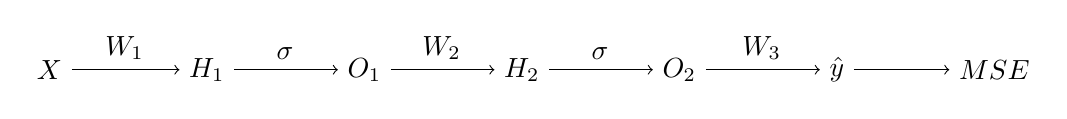
\begin{tikzpicture}
	\tikzstyle{place}=[rectangle, draw=black, minimum size = 8mm]
	\draw node at (0, 0) (input) {$X$};
	\draw node at (2, 0) (h1) {$H_1$};
	\draw node at (4, 0) (o1) {$O_1$};
	\draw node at (6, 0) (h2) {$H_2$};
	\draw node at (8, 0) (o2) {$O_2$};
	\draw node at (10, 0) (output) {$\hat{y} $};
	\draw node at (12, 0) (mse) {$MSE$};
	
	\draw [->]  (input) -- (h1) node[pos=.49, above] {$W_1$} ;
	\draw [->]  (h1) -- (o1) node[pos=.49, above] {$\sigma$} ;
	\draw [->]  (o1) -- (h2) node[pos=.49, above] {$W_2$} ;
	\draw [->]  (h2) -- (o2) node[pos=.49, above] {$\sigma$} ;
	\draw [->]  (o2) -- (output) node[pos=.49, above] {$W_3$} ;
	\draw [->]  (output) to (mse);	
	\end{tikzpicture}
\end{center}

Обратный проход по нейронной сети (backward pass):

\begin{center}
	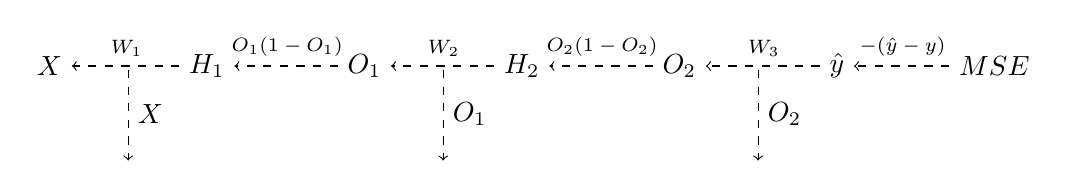
\begin{tikzpicture}
	\draw node at (0, 0) (input) {$X$};
	\draw node at (2, 0) (h1) {$H_1$};
	\draw node at (4, 0) (o1) {$O_1$};
	\draw node at (6, 0) (h2) {$H_2$};
	\draw node at (8, 0) (o2) {$O_2$};
	\draw node at (10, 0) (output) {$\hat{y}$};
	\draw node at (12, 0) (mse) {$MSE$};
	
	\draw [->, dashed]   (h1)  -- (input) node[pos=.49, above] {\scriptsize $W_1$} ;
	\draw [->, dashed]   (o1) -- (h1) node[pos=.49, above] {\scriptsize $O_1 (1-O_1)$} ;
	\draw [->, dashed]   (h2) -- (o1) node[pos=.49, above] {\scriptsize $W_2$} ;
	\draw [->, dashed]   (o2) -- (h2) node[pos=.49, above] {\scriptsize $O_2 (1 - O_2)$} ;
	\draw [->, dashed]   (output) -- (o2)node[pos=.49, above] {\scriptsize $W_3$} ;
	\draw [->, dashed]  (mse) -- (output) node[pos=.49, above] {\scriptsize $-(\hat{y} - y)$} ;	
	
	\draw [->, dashed]  (9, -0.05) -- (9, -1.2)  node[pos=.49, right] {$O_2$} ;
	\draw [->, dashed]  (5, -0.05) -- (5, -1.2)  node[pos=.49, right] {$O_1$} ;
	\draw [->, dashed]  (1, -0.05) -- (1, -1.2)  node[pos=.49, right] {$X$} ;
	\end{tikzpicture}
\end{center}

По аналогии с предыдущей задачей выпишем формулы для обратного распространения ошибки:

\begin{minipage}{.2\linewidth}
	\begin{equation*} 
		\begin{aligned}
			&  d = - (\hat{y} - y) \\
			&  \frac{\partial MSE}{\partial W_3} = d \cdot O_2  \\
		\end{aligned}
	\end{equation*}
\end{minipage} \hfill
\begin{minipage}{.35\linewidth}
	\begin{equation*} 
		\begin{aligned}
			&  d = d \cdot W_3 \cdot O_2 \cdot (1 - O_2)  \\
			&  \frac{\partial MSE}{\partial W_2} = d \cdot O_1 \\
		\end{aligned}
	\end{equation*}
\end{minipage} \hfill
\begin{minipage}{.35\linewidth}
	\begin{equation*} 
	\begin{aligned}
	&  d = d \cdot W_2 \cdot O_1 \cdot (1 - O_1)  \\
	&  \frac{\partial MSE}{\partial W_1} = d \cdot X \\
	\end{aligned}
	\end{equation*}
\end{minipage}

Когда мы аккуратно подставим все числа, можно будет сделать шаг SGD

\begin{minipage}{.28\textwidth}
    \[  W_3^t = W_3^{t-1} - \eta \cdot \frac{\partial MSE}{\partial W_3}  \]
\end{minipage}
\begin{minipage}{.3\textwidth}
	\[  W_2^t = W_2^{t-1} - \eta \cdot \frac{\partial MSE}{\partial W_2}  \]
\end{minipage}
\begin{minipage}{.35\textwidth}
	\[  W_1^t = W_1^{t-1} - \eta \cdot \frac{\partial MSE}{\partial W_1}  \]
\end{minipage}

Начинаем проворачивать алгоритм. Делаем прямое распространение для второго наблюдения, напомним, что матрицы весов инициализированы нулями:

\begin{center}
	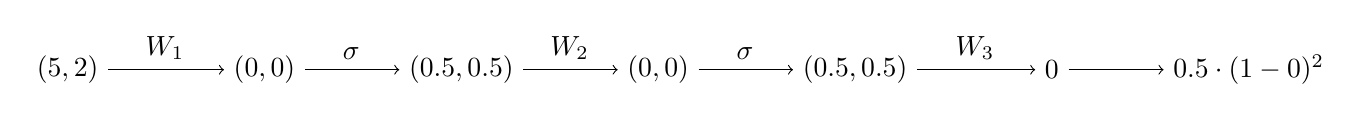
\begin{tikzpicture}
	\tikzstyle{place}=[rectangle, draw=black, minimum size = 8mm]
	\draw node at (0, 0) (input) {$(5, 2)$};
	\draw node at (2.5, 0) (h1) {$(0, 0)$};
	\draw node at (5, 0) (o1) {$(0.5, 0.5)$};
	\draw node at (7.5, 0) (h2) {$(0, 0)$};
	\draw node at (10, 0) (o2) {$(0.5, 0.5)$};
	\draw node at (12.5, 0) (output) {$0$};
	\draw node at (15, 0) (mse) {$0.5 \cdot (1 - 0)^2$};
	
	\draw [->]  (input) -- (h1) node[pos=.49, above] {$W_1$} ;
	\draw [->]  (h1) -- (o1) node[pos=.49, above] {$\sigma$} ;
	\draw [->]  (o1) -- (h2) node[pos=.49, above] {$W_2$} ;
	\draw [->]  (h2) -- (o2) node[pos=.49, above] {$\sigma$} ;
	\draw [->]  (o2) -- (output) node[pos=.49, above] {$W_3$} ;
	\draw [->]  (output) to (mse);	
	\end{tikzpicture}
\end{center}

Делаем обратный проход. \textbf{Шаг 1:}

\begin{equation*} 
	\begin{aligned}
		&  d = - (\hat{y} - y) = -1 \\
		&  \frac{\partial MSE}{\partial W_3} = d \cdot O_2 = -1 \cdot (0.5, 0.5) = (-0.5, -0.5) \\
	\end{aligned}
\end{equation*}
	
\textbf{Шаг 2:}

\begin{equation*} 
	\begin{aligned}
		&  d = d \cdot W_3 \cdot O_2 \cdot (1 - O_2) = -1 \cdot \begin{pmatrix} 0 \\ 0 \end{pmatrix} \cdot (0.5, 0.5) \cdot (0.5, 0.5) \\
		&  \frac{\partial MSE}{\partial W_2} = d \cdot O_1 \\
	\end{aligned}
\end{equation*}


\textbf{Шаг 3:}

\begin{equation*} 
	\begin{aligned}
    	&  d = d \cdot W_2 \cdot O_1 \cdot (1 - O_1)  \\
    	&  \frac{\partial MSE}{\partial W_1} = d \cdot X \\
	\end{aligned}
\end{equation*}

\end{sol} 
















%%%-------------------------------------------
% \begin{problem}{(Backpropagation своими руками)}
%     Маша как-то раз решала задачу классифкации. С тех пор у неё в кармане завалялась нейросеть: 

% 	\begin{center}
% 		\begin{tikzpicture}[scale = 1.5, line cap=round,line join=round,x=1.0cm,y=1.0cm]
% 		\clip(-4.624679143882289,1.3686903642723092) rectangle (3.8521836267384844,4.8154607149701345);
% 		\draw [line width=2.pt] (-2.5,2.5) circle (0.5cm);
% 		\draw [line width=2.pt] (-0.5,2.5) circle (0.5cm);
% 		\draw [line width=2.pt] (1.5,2.5) circle (0.5cm);
% 		\draw [->,line width=2.pt] (-3.5,4.) -- (-2.831496141146421,2.874313115459547);
% 		\draw [->,line width=2.pt] (-4.,2.5) -- (-3.,2.5);
% 		\draw [->,line width=2.pt] (-2.,2.5) -- (-1.,2.5);
% 		\draw [->,line width=2.pt] (0.,2.5) -- (1.,2.5);
% 		\draw [->,line width=2.pt] (2.,2.5) -- (3.,2.5);
% 		\draw [->,line width=2.pt] (-1.5,4.) -- (-0.8294354120380936,2.8761280490674572);
% 		\draw [->,line width=2.pt] (0.5,4.) -- (1.1775032003746246,2.8820939861230355);
% 		\draw (-3.686865302879703,4.5) node[anchor=north west] {$1$};
% 		\draw (-1.67726421501702,4.5) node[anchor=north west] {$1$};
% 		\draw (0.2957986712481599,4.5) node[anchor=north west] {$1$};
% 		\draw (-4.320194130569761,2.805859627107445) node[anchor=north west] {$x$};
% 		\draw (3.1214195947884176,2.7693214255099416) node[anchor=north west] {$y$};
% 		\draw (-3.7112241039447054,3.07380643882247) node[anchor=north west] {$w_1^1$};
% 		\draw (-3.114433477852151,3.9750820782275555) node[anchor=north west] {$w_0^1$};
% 		\draw (-1.7138024166145234,3.122524040952475) node[anchor=north west] {$w_1^2$};
% 		\draw (-1.1535499921194723,4.13341428515007) node[anchor=north west] {$w_0^2$};
% 		\draw (1.0387421037307276,4.109055484085068) node[anchor=north west] {$w_0^3$};
% 		\draw (0.2836192707156588,3.0859858393549713) node[anchor=north west] {$w_1^3$};
% 		\end{tikzpicture}
% 	\end{center} 
	
% 	В качестве функции активации Маша использовала сигмоиду: $f(t) = \frac{e^t}{1 + e^t}$.  Как это обычно бывает, Маша обнаружила её в своих штанах после стирки и очень обрадовалась. Теперь она хочет сделать два шага стохастического градиентного спуска, используя алгоритм обратного распространения ошибки.
	
% 	У неё есть два наблюдения: $x_1 = 1, x_2 = 5$, $y_1 =1$, $y_2 = 0$. Скорость обучения $\gamma = 1$. В качестве инициализации взяты нулевые веса. Сначала берётся второе наблюдение, затем первое. Помогите Маше. 
% \end{problem}

% %%%-------------------------------------------
% \begin{problem}{(Незаметный backpropagation)}
%     Маша собрала нейросеть: 
	
% 	\begin{equation*}
% 	y =   \max \left( 0;  X \cdot  \begin{pmatrix} 1 & -1 \\ 0.5 & 0 \end{pmatrix} \right) \cdot \begin{pmatrix} 0.5 \\ 1 \end{pmatrix} 
% 	\end{equation*}

% 	Теперь Маша внимательно смотрит на неё.
	
% 	\begin{enumerate}
% 		\item  Первый слой нашей нейросетки --- линейный. По какой формуле делается forward pass? Предположим, что на вход пришло наблюдение $x = (1, 2)$. Сделайте через этот слой forward pass и найдите выход из слоя.
		
% 		\item Найдите для первого слоя производную выхода по входу. При обратном движении по нейросетке, в первый слой пришёл накопленный градиент $(-1, 0)$. Каким будет новое накопленное значение градиента, которое выплюнет из себя линейный слой? По какой формуле делается backward pass? 
		
% 		\item Второй слой нейросетки ---- функция активации, $ReLU.$  По какой формуле делается forward pass? На вход в него поступило значение $(2, -1)$. Сделайте через него forward pass. 
		
% 		\item Найдите для второго слоя производную выхода по входу. При обратном движении по нейросетке во второй слой пришёл накопленный градиент $(-1, -2)$.  Каким будет новое накопленное значение градиента, которое выплюнет из себя $ReLU$?  По какой формуле делается backward pass? 
		
% 		\item Третий слой нейросетки --- линейный.  По какой формуле делается forward pass? Пусть на вход поступило значение $(2,0)$.  Сделайте через него forward pass. 
		
% 		\item Найдите для третьего слоя производную выхода по входу. При обратном движении по нейросетке, в третий слой пришёл накопленный градиент $-2$. Каким будет новое накопленное значение градиента, которое выплюнет из себя линейный слой?  По какой формуле делается backward pass? 
% 		\item Мы решаем задачу Регрессии. В качестве функции ошибки мы используем $MSE$. Пусть для рассматриваемого наблюдения реальное значение $y = 0$. Найдите значение $MSE$. Чему равна производная $MSE$ по входу (прогнозу)? Каким будет накопленное значение градиента, которое $MSE$ выплюнет из себя в предыдущий слой нейросетки, если изначально значение градиента инициализировано единицей? 
		
% 		\item Пусть скорость обучения $\gamma = 1$.  Сделайте для весов нейросети шаг градиентного спуска. 
% 	\end{enumerate}

% 	Посидела Маша, посидела, и поняла, что неправильно она всё делает. В реальности перед ней не задача регрессии, а задача классификации. 
	
% 	\begin{enumerate}	
% 		\item Маша навинтила поверх второго линейного слоя сигмоиду. Как будет для неё выглядеть forward pass? Сделайте его. Найдите для сигмоиды производную выхода по входу.
		
% 		\item В качестве функции потерь Маша использует $\logloss.$ Как для этой функции потерь выглядит forward pass? Сделайте его. Найдите для $\logloss$ производную выхода по входу. 
		
% 		\item Как будет выглядеть backward pass через $logloss$ и сигмоиду? Прделайте его. Как изменится процедура градиентного спуска для остальной части сети? 
% 	\end{enumerate}
% \end{problem} 


% %%%-------------------------------------------
% \begin{problem}{(Ещё один backpropagation)}
%     У Маши есть трёхслойная нейросеть: 
    
% 	$$ 
% 	y = f(f(X \cdot W_3 ) \cdot W_2) \cdot W_1 
% 	$$
	
% 	\begin{enumerate} 
% 	    \item Маща использует в качестве функции активации $f(t) = ReLU(t) =  \max(0; t)$, а в качестве функции потерь $L(W_1, W_2) = \frac{1}{2} \cdot (y - \hat y)^2$.
	    
% 	    \item 
	    
	    
% 	    \item 
	    
% 	    \item 
	
% 	\end{enumerate}
	
% 	Для всех пунктов запишите уравнения для прямого и обратного проходов по сетке. Выпишите для всех весов уравнения, по которым будет делаться шаг градиентного спуска. 
% \end{problem} 


% %%%--------------------------------------------
% \begin{problem}{(Нестеров и backprop)}

%     \todo[inline]{Найти про это какую-нибудь статью}
    
%     К Маше приехал её папа и загрузил её интересным вопросом. В алгоритме обратного распространения ошибки мы можем делать шаг как минимум двумя способами: 
    
%     \begin{enumerate} 
%         \item Зафиксировали все $w_{t-1},$ нашли все градиенты, сделали сразу по всем весам шаг градиентного спуска.
        
%         \item Нашли градиенты для последнего слоя и сделали шаг для его весов, получили $w_t^k.$ Для поиска градиентов предпоследнего слоя используем веса  $w_t^k,$ а не $w_{t-1}^k.$ Все остальные слои обновляем по аналогии. 
%     \end{enumerate} 
    
%     Как думаете, какой из способов будет приводить к более быстрой сходимости и почему? 
% \end{problem} 









%-----------------------------------

% \begin{center}
% 	\begin{tikzpicture}
% 	\draw node at (0, 0) (input) {$X$};
% 	\draw node at (2, 0) (h1) {$H_1$};
% 	\draw node at (4, 0) (o1) {$O_1$};
	
% 	\only<3>{ 
% 		\draw node at (0, 0) (input) {\color{red} $X$};
% 		\draw node at (2, 0) (h1) {\color{red} $H_1$};
% 		\draw node at (4, 0) (o1) {\color{red} $O_1$};
% 	}
	
% 	\draw node at (6, 0) (h2) {$H_2$};
% 	\draw node at (8, 0) (o2) {$O_2$};
	
% 	\only<2>{ 
% 		\draw node at (6, 0) (h2) {\color{red}  $H_2$};
% 		\draw node at (8, 0) (o2) {\color{red} $O_2$};	
% 	}
	
% 	\draw node at (10, 0) (output) {$\hat{y}$};
% 	\draw node at (12, 0) (mse) {$MSE$};
	
% 	\only<1>{ 
% 		\draw node at (10, 0) (output) {\color{red} $\hat{y}$};
% 		\draw node at (12, 0) (mse) {\color{red} $MSE$};	
% 	}
		
% 	\draw [->, dashed]   (output) -- (o2)node[pos=.49, above] {\scriptsize $W_3$} ;
% 	\draw [->, dashed]  (mse) -- (output) node[pos=.49, above] {\scriptsize $-2(\hat{y} - y)$} ;	
% 	\draw [->, dashed]  (9, -0.05) -- (9, -1.2)  node[pos=.49, right] {$O_2$} ;
		
% 	\only<1>{ 
% 		\draw [->, dashed, red]   (output) -- (o2)node[pos=.49, above] {\color{red} \scriptsize $W_3$} ;
% 		\draw [->, dashed, red]  (mse) -- (output) node[pos=.49, above] {\color{red} \scriptsize $-2(\hat{y} - y)$} ;	
% 		\draw [->, dashed, red]  (9, -0.05) -- (9, -1.2)  node[pos=.49, right] {\color{red} $O_2$} ;
% 	}

% 	\draw [->, dashed]   (h2) -- (o1) node[pos=.49, above] {\scriptsize $W_2$} ;
% 	\draw [->, dashed]   (o2) -- (h2) node[pos=.49, above] {\scriptsize $O_2 (1 - O_2)$} ;
% 	\draw [->, dashed]  (5, -0.05) -- (5, -1.2)  node[pos=.49, right] {$O_1$} ;
	
% 	\only<2>{ 
% 		\draw [->, dashed, red]   (h2) -- (o1) node[pos=.49, above] {\color{red} \scriptsize $W_2$} ;
% 		\draw [->, dashed, red]   (o2) -- (h2) node[pos=.49, above] {\color{red} \scriptsize $O_2 (1 - O_2)$} ;
% 		\draw [->, dashed, red]  (5, -0.05) -- (5, -1.2)  node[pos=.49, right] {\color{red} $O_1$} ;
% 	}

% 	\draw [->, dashed]   (h1)  -- (input) node[pos=.49, above] {\scriptsize $W_1$} ;
% 	\draw [->, dashed]   (o1) -- (h1) node[pos=.49, above] {\scriptsize $O_1 (1-O_1)$} ;
% 	\draw [->, dashed]  (1, -0.05) -- (1, -1.2)  node[pos=.49, right] {$X$} ;

% 	\only<3>{ 
% 		\draw [->, dashed, red]   (h1)  -- (input) node[pos=.49, above] {\color{red} \scriptsize $W_1$} ;
% 		\draw [->, dashed, red]   (o1) -- (h1) node[pos=.49, above] {\color{red} \scriptsize $O_1 (1-O_1)$} ;
% 		\draw [->, dashed, red]  (1, -0.05) -- (1, -1.2)  node[pos=.49, right] {\color{red} $X$} ;
% 	}	
% 	\end{tikzpicture}
% \end{center}

% \vfill

% \begin{columns}
% 	\begin{column}{.28\textwidth}
% 		\alert{Шаг 1:}
% 		\begin{equation*} 
% 			\begin{aligned}
% 				&  d = -2 (\hat{y} - y) \\
% 				&  \frac{\partial MSE}{\partial W_3} = d \cdot O_2  \\
% 			\end{aligned}
% 		\end{equation*}
% 	\end{column}
% 	\begin{column}{.3\textwidth}
% 		\only<2-3>{
% 		\alert{Шаг 2:}
% 		\begin{equation*} 
% 			\begin{aligned}
% 				&  d = d \cdot W_3 \cdot O_2 \cdot (1 - O_2)  \\
% 				&  \frac{\partial MSE}{\partial W_2} = d \cdot O_1 \\
% 			\end{aligned}
% 		\end{equation*}}
% 	\end{column}
% 	\begin{column}{.35\textwidth}
% 		\only<3>{
% 		\alert{Шаг 3:}
% 		\begin{equation*} 
% 		\begin{aligned}
% 		&  d = d \cdot W_2 \cdot O_1 \cdot (1 - O_1)  \\
% 		&  \frac{\partial MSE}{\partial W_1} = d \cdot X \\
% 		\end{aligned}
% 		\end{equation*}}
% 	\end{column}
% \end{columns}
